\documentclass{beamer}

% \usepackage{beamerthemesplit} // Activate for custom appearance


%Unnumbered footnotes
\newcommand\ufoot[1]{
\begingroup
\renewcommand\thefootnote{}\footnote{#1}
\addtocounter{footnote}{-1}
\endgroup
}


\title{placeholder}
\subtitle{IB 516 Analytical Workflows}
\author{Ben Dalziel}
\date{\today}

\begin{document}

\frame{\titlepage}

\section[Outline]{}

\frame{
	\frametitle{Outline}
	\tableofcontents
}

\section{Introduction to Version Control}

\frame{
	\frametitle{What is a version control system?}

	A version control system (VCS) records changes in a set of files over time so that you can recall specific versions later.
	A VCS allows:
	-'time travel' back and forth from any previous time in your project development.
	-peaceful coexistence and exchange of info between 'parallel universes' of a project
	
	In science this is about organizing stable efficient collaborations (with others and with your past self) that produce reproducible work.
}


\frame{
	\frametitle{In practice}
	
	revert selected files back to a previous state
	revert the entire project back to a previous state
	compare changes over time
	see who last modified something that might be causing a problem, who introduced an issue and when, and more. 
	if you screw things up or lose files, you can easily recover. 
	
	you get all this for very little overhead.
	
	\ufoot{\tiny{https://git-scm.com/book/en/v2/Getting-Started-About-Version-Control}}

}
	


\frame{
	\frametitle{Visualizing a version controlled project through time}
	
	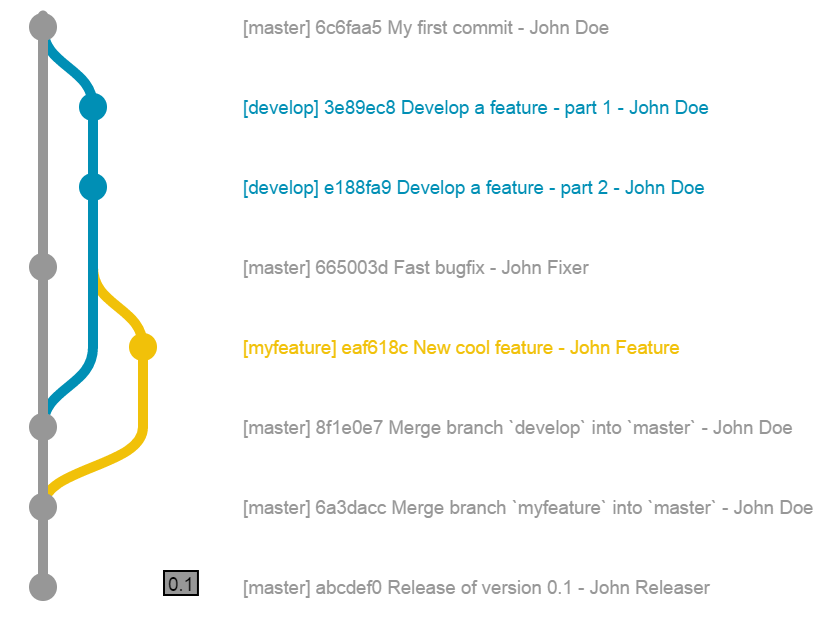
\includegraphics[scale = 0.3]{figs/pretty_branch_graph}
	
	\ufoot{\tiny{https://stackoverflow.com/a/24107223}}


}



\frame{
	\frametitle{Version control in Git: How Git stores data}
	
	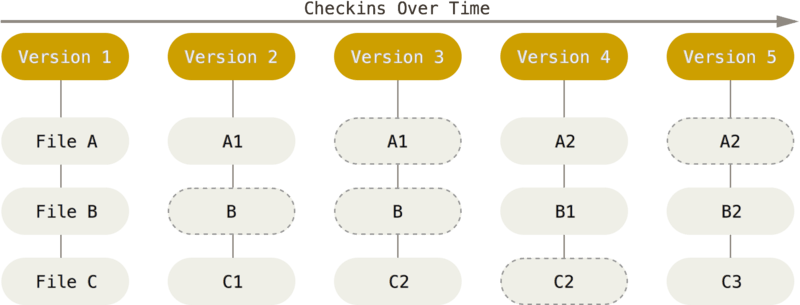
\includegraphics[scale = 0.4]{figs/how_git_stores_data}
	
	\ufoot{\tiny{http://git-scm.com/book/en/v2/Getting-Started-What-is-Git}}
	
	
}




\section{Basic Workflow}


\frame{
	\frametitle{Basic lifecyle of work on a file}
	
	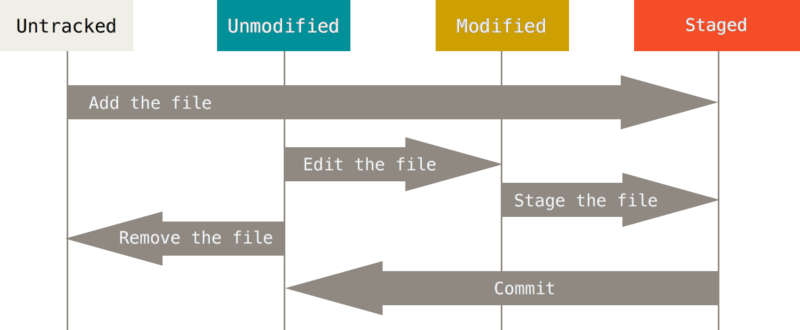
\includegraphics[scale = 0.4]{figs/lifecycle}
		
	\ufoot{\tiny{http://git-scm.com/book/en/v2/Getting-Started-What-is-Git}}
	
	\tiny{*We haven't talked about $staging$ which is an intermediate step between modifying a file and commiting it. Git allows you to choose which modified files will be part of the next commit. Typically we will want to commit all modifications and Github Desktop automatically stages all modifications, so we don't need to think too much about staging at the moment.}
	
}


	

\frame{
	\frametitle{Git words}
	
	so far:
	repository, commit, push, fetch, merge, pull, local, origin, master, branch, fork
	
	
}


\frame{
	\frametitle{Naming commits}

	

}
	
